% This is "aamas2015_sample.tex", a revised version of aamas2014_sample.tex
% This file should be compiled with "aamas2015.cls" 
% This example file demonstrates the use of the 'aamas2015.cls'
% LaTeX2e document class file. It is intended for those submitting
% articles to the AAMAS-2015 conference. This file is based on
% the sig-alternate.tex example file.
% The 'sig-alternate.cls' file of ACM will produce a similar-looking,
% albeit, 'tighter' paper resulting in, invariably, fewer pages
% than the original ACM style.
%
% ----------------------------------------------------------------------------------------------------------------
% This .tex file (and associated .cls ) produces:
%       1) The Permission Statement
%       2) The Conference (location) Info information
%       3) The Copyright Line with AAMAS data
%       4) NO page numbers
%
% as against the acm_proc_article-sp.cls file which
% DOES NOT produce 1) through 3) above.
%
% Using 'aamas2015.cls' you don't have control
% from within the source .tex file, over both the CopyrightYear
% (defaulted to 20XX) and the IFAAMAS Copyright Data
% (defaulted to X-XXXXX-XX-X/XX/XX).
% These information will be overwritten by fixed AAMAS 2015  information
% in the style files - it is NOT as you are used to with ACM style files.
%
% ---------------------------------------------------------------------------------------------------------------
% This .tex source is an example which *does* use
% the .bib file (from which the .bbl file is produced).
% REMEMBER HOWEVER: After having produced the .bbl file,
% and prior to final submission, you *NEED* to 'insert'
% your .bbl file into your source .tex file so as to provide
% ONE 'self-contained' source file.
%


\documentclass{aamas2015}

% if you are using PDF LaTeX and you cannot find a way for producing
% letter, the following explicit settings may help

\usepackage{pdfsync}
\usepackage{comment}
\usepackage{amsmath}
\usepackage{amssymb}
\usepackage{amsbsy}
%\usepackage{amsthm}
\usepackage{calc}
\usepackage{color}
\usepackage{url}
\usepackage{xspace}
%\usepackage[caption=false]{subfig}
\usepackage{subfigure}
\usepackage{graphicx}
\usepackage{xcolor}
\usepackage{comment}
\usepackage{xspace}
\usepackage{tikz}
\usepackage{epsdice}
\usetikzlibrary{trees}
\usetikzlibrary{shapes.geometric}
\tikzset{
  treenode/.style = {align=center, inner sep=0pt, font=\sffamily},
  ma/.style = {draw,treenode, shape border rotate=90, isosceles triangle,isosceles triangle apex angle=60, black, minimum width=2mm},% arbre rouge noir, noeud noir
  mi/.style = {ma, shape border rotate=-90},
  ch/.style = {draw, treenode, circle, minimum width=2mm, black}
}

\tikzstyle{level 1}=[level distance=8mm, sibling distance=1.5cm]
\tikzstyle{level 2}=[level distance=8mm, sibling distance=1cm]
\tikzstyle{level 3}=[level distance=8mm, sibling distance=0.5cm]

\usepackage[algo2e, noend, noline, linesnumbered]{algorithm2e}
\providecommand{\SetAlgoLined}{\SetLine}  
\providecommand{\DontPrintSemicolon}{\dontprintsemicolon}
\DontPrintSemicolon
\makeatletter
\newcommand{\pushline}{\Indp}% Indent
\newcommand{\popline}{\Indm}
\makeatother

% the note center!
\definecolor{darkgreen}{RGB}{0,125,0}
\newcounter{vlNoteCounter}
\newcounter{mlNoteCounter}
\newcounter{mbNoteCounter}
\newcommand{\vlnote}[1]{{\scriptsize \color{blue} $\blacksquare$ \refstepcounter{vlNoteCounter}\textsf{[VL]$_{\arabic{vlNoteCounter}}$:{#1}}}}
\newcommand{\mlnote}[1]{{\scriptsize \color{darkgreen} $\blacksquare$ \refstepcounter{mlNoteCounter}\textsf{[ML]$_{\arabic{mlNoteCounter}}$:{#1}}}}
\newcommand{\asnote}[1]{{\scriptsize \color{red} $\blacktriangle$ \refstepcounter{mbNoteCounter}\textsf{[MB]$_{\arabic{asNoteCounter}}$:{#1}}}}

\renewcommand{\vlnote}[1]{}
\renewcommand{\mlnote}[1]{}
\renewcommand{\asnote}[1]{}


\newcommand{\argmin}{\operatornamewithlimits{argmin}}
\newcommand{\argmax}{\operatornamewithlimits{argmax}}
\newcommand{\bE}{\mathbb{E}}
\newcommand{\bx}{\mathbf{x}}
\newcommand{\bg}{\mathbf{g}}
\newcommand{\bu}{\mathbf{u}}
\newcommand{\bU}{\mathbf{U}}
\newcommand{\cI}{\mathcal{I}}
\newcommand{\cC}{\mathcal{C}}
\newcommand{\tta}{\mathtt{a}}
\newcommand{\ttm}{\mathtt{m}}
\newcommand{\PW}{\mbox{PW}}
\newcommand{\BR}{\mbox{BR}}
\newcommand{\defword}[1]{\textbf{\boldmath{#1}}}
\newcommand{\ie}{{\it i.e.}~}
\newcommand{\eg}{{\it e.g.}~}
\newtheorem{definition}{Definition}
\newtheorem{fact}{Fact}
\newtheorem{theorem}{Theorem}
\newtheorem{corollary}{Corollary}
\newtheorem{lemma}{Lemma}
\newtheorem{proposition}{Proposition}
\newcommand{\Proof}{{\noindent\bf Proof. }}
\newcommand{\citejustyear}[1]{\cite{#1}}
\newcommand{\Qed}{$\blacksquare$}
\newcommand{\abs}[1]{\left|#1\right|}
\newcommand{\todo}[1]{{\color{red}{\bf #1}}}
\newcommand{\breturn}{{\bf return}\xspace}
 
\pdfpagewidth=8.5truein
\pdfpageheight=11truein

\begin{document}

% In the original styles from ACM, you would have needed to
% add meta-info here. This is not necessary for AAMAS 2015  as
% the complete copyright information is generated by the cls-files.

\title{Online Monte Carlo Counterfactual Regret Minimization for Search in Imperfect Information Games}

% AUTHORS


% For initial submission, do not give author names, but the
% tracking number, instead, as the review process is blind.

% You need the command \numberofauthors to handle the 'placement
% and alignment' of the authors beneath the title.
%
% For aesthetic reasons, we recommend 'three authors at a time'
% i.e. three 'name/affiliation blocks' be placed beneath the title.
%
% NOTE: You are NOT restricted in how many 'rows' of
% "name/affiliations" may appear. We just ask that you restrict
% the number of 'columns' to three.
%
% Because of the available 'opening page real-estate'
% we ask you to refrain from putting more than six authors
% (two rows with three columns) beneath the article title.
% More than six makes the first-page appear very cluttered indeed.
%
% Use the \alignauthor commands to handle the names
% and affiliations for an 'aesthetic maximum' of six authors.
% Add names, affiliations, addresses for
% the seventh etc. author(s) as the argument for the
% \additionalauthors command.
% These 'additional authors' will be output/set for you
% without further effort on your part as the last section in
% the body of your article BEFORE References or any Appendices.

%\numberofauthors{8} %  in this sample file, there are a *total*
% of EIGHT authors. SIX appear on the 'first-page' (for formatting
% reasons) and the remaining two appear in the \additionalauthors section.
%

\numberofauthors{1}

\author{
% You can go ahead and credit any number of authors here,
% e.g. one 'row of three' or two rows (consisting of one row of three
% and a second row of one, two or three).
%
% The command \alignauthor (no curly braces needed) should
% precede each author name, affiliation/snail-mail address and
% e-mail address. Additionally, tag each line of
% affiliation/address with \affaddr, and tag the
% e-mail address with \email.
% 1st. author
\alignauthor
Paper XXX
%Ben Trovato\titlenote{Dr.~Trovato insisted his name be first.}\\
%       \affaddr{Institute for Clarity in Documentation}\\
%       \affaddr{1932 Wallamaloo Lane}\\
%       \affaddr{Wallamaloo, New Zealand}\\
%       \email{trovato@corporation.com}
% 2nd. author
%\alignauthor
%G.K.M. Tobin\titlenote{The secretary disavows any knowledge of this author's actions.}\\
%       \affaddr{Institute for Clarity in Documentation}\\
%       \affaddr{P.O. Box 1212}\\
%       \affaddr{Dublin, Ohio 43017-6221}\\
%       \email{webmaster@marysville-ohio.com}
% 3rd. author
%\alignauthor Lars Th{\o}rv{\"a}ld\titlenote{This author is the one who did all the really hard work.}\\
%       \affaddr{The Th{\o}rv{\"a}ld Group}\\
%       \affaddr{1 Th{\o}rv{\"a}ld Circle}\\
%       \affaddr{Hekla, Iceland}\\
%       \email{larst@affiliation.org}
}

%\and  % use '\and' if you need 'another row' of author names

% 4th. author
%\alignauthor Lawrence P. Leipuner\\
%       \affaddr{Brookhaven Laboratories}\\
%       \affaddr{Brookhaven National Lab}\\
%       \affaddr{P.O. Box 5000}\\
%       \email{lleipuner@researchlabs.org}

% 5th. author
%\alignauthor Sean Fogarty\\
%       \affaddr{NASA Ames Research Center}\\
%       \affaddr{Moffett Field}\\
%       \affaddr{California 94035}\\
%       \email{fogartys@amesres.org}

% 6th. author
%\alignauthor Charles Palmer\\
%       \affaddr{Palmer Research Laboratories}\\
%      \affaddr{8600 Datapoint Drive}\\
%       \affaddr{San Antonio, Texas 78229}\\
%       \email{cpalmer@prl.com}

%\and

%% 7th. author
%\alignauthor Lawrence P. Leipuner\\
%       \affaddr{Brookhaven Laboratories}\\
%       \affaddr{Brookhaven National Lab}\\
%       \affaddr{P.O. Box 5000}\\
%       \email{lleipuner@researchlabs.org}

%% 8th. author
%\alignauthor Sean Fogarty\\
%       \affaddr{NASA Ames Research Center}\\
%       \affaddr{Moffett Field}\\
%       \affaddr{California 94035}\\
%       \email{fogartys@amesres.org}

%% 9th. author
%\alignauthor Charles Palmer\\
%       \affaddr{Palmer Research Laboratories}\\
%       \affaddr{8600 Datapoint Drive}\\
%       \affaddr{San Antonio, Texas 78229}\\
%       \email{cpalmer@prl.com}

%}

%% There's nothing stopping you putting the seventh, eighth, etc.
%% author on the opening page (as the 'third row') but we ask,
%% for aesthetic reasons that you place these 'additional authors'
%% in the \additional authors block, viz.
%\additionalauthors{Additional authors: John Smith (The Th{\o}rv{\"a}ld Group,
%email: {\texttt{jsmith@affiliation.org}}) and Julius P.~Kumquat
%(The Kumquat Consortium, email: {\texttt{jpkumquat@consortium.net}}).}
%\date{30 July 1999}
%% Just remember to make sure that the TOTAL number of authors
%% is the number that will appear on the first page PLUS the
%% number that will appear in the \additionalauthors section.

\maketitle

\begin{abstract}
Online search in games has been a core interest of artificial intelligence. 
%Advances made in search for perfect information games 
%have led to AI capable of defeating the world's top human experts. 
Search in imperfect information games (\eg Poker, Bridge, Skat) is particularly challenging due to 
the complexities introduced by hidden information.  
In this paper, we present Online Outcome Sampling, 
an online search variant of Monte Carlo Counterfactual Regret Minimization, which preserves its convergence to Nash equilibrium.
We show that OOS can overcome the problem of non-locality encountered by previous search algorithms and perform well against its worst case opponents.
We show that exploitability of the strategies played by OOS decreases as
the amount of search time increases, and that Information Set Monte Carlo tree search can remain exploitable or get more exploitable over time.
In head-to-head play, OOS outperforms ISMCTS in games where non-locality plays a significant role, given a sufficient computation time per move.
\end{abstract}

% Note that the category section should be completed after reference to the ACM Computing Classification Scheme available at
% http://www.acm.org/about/class/1998/.

%\category{H.4}{Information Systems Applications}{Miscellaneous}

%A category including the fourth, optional field follows...
%\category{D.2.8}{Software Engineering}{Metrics}[complexity measures, performance measures]

%General terms should be selected from the following 16 terms: Algorithms, Management, Measurement, Documentation, Performance, Design, Economics, Reliability, Experimentation, Security, Human Factors, Standardization, Languages, Theory, Legal Aspects, Verification.

%\terms{Delphi theory}

%Keywords are your own choice of terms you would like the paper to be indexed by.

%\keywords{AAMAS proceedings, \LaTeX, text tagging}

\section{Introduction}

Algorithms for creating strong strategies in games have been a core interest of artificial intelligence research. Strong strategies are useful not only as research benchmarks and as challenging opponents in digital entertainment, but they are becoming increasingly important also in real world applications, such as critical infrastructure security~\cite{Tambe11}.
Because these games are often played against unknown opponents, a good strategy should be sufficiently robust against any possible counterstrategy used by the adversary. In strictly competitive games, the strategy that is optimal with respect to the robustness against any opponent is the Nash equilibrium. It is guaranteed to provide the maximal possible expected value against any strategy of the opponent. For example, an equilibrium defense strategy could minimize the maximal damage caused by an adversary's attack.

When preparation time is abundant and the exact problem definition is known in advance, an equilibrium strategy for a smaller abstract game can be pre-computed and 
then used during game play. This {\it offline approach} has been remarkably successful in 
Computer Poker \cite{Johanson07Msc,Gilpin09,Sandholm10The,Rubin11Poker,Johanson13Evaluating}. 
%and it is also prevalent used in the security applications~\cite{XXX} \mlnote{Citation needed; also, we may be appealing a bit too much to the security domain given the content of the rest of the paper.. maybe just remove this?}. Removed for now.
However, the preparation time is often very limited. The model of the game may become known only shortly before acting is necessary, such as in general game-playing, search or pursuit in a previously unknown environment, and general-purpose robotics. In these circumstances, creating and solving an abstract representation of the problem may not be possible. In these cases, agents must {\it decide online}: make initial decisions quickly and then spend effort to improve their strategy while the interaction is taking place.

In this paper, we propose a search algorithm that can compute an approximate Nash equilibrium (NE) strategy in two-player zero-sum games {\it online}, in a previously unknown game, with a very limited computation time. 
We introduce Online Outcome Sampling (OOS), a simulation-based algorithm based on Monte Carlo Counterfactual Regret Minimization~(MCCFR)~\cite{Lanctot09Sampling}. 
% (not sure we need this, and I'm sure reviewers already know) a popular offline equilibrium solving algorithm for this class of games. 
%In order to use computational time and space efficiently,
OOS makes two novel modifications to MCCFR. First, OOS builds its search tree incrementally, like Monte Carlo tree search 
(MCTS)~\cite{Coulom06Efficient,mctssurvey,UCT}. Second, when performing additional computation after some moves have been played in the match, the following samples are targeted primarily to the parts of the game tree, which are more relevant to the current situation in the game.
We show that OOS is {\it consistent}, \ie it is guaranteed to converge to an equilibrium strategy as search time increases. To the best of our knowledge, this is not the case for any existing online game playing algorithm. This is possible because OOS is the first algorithm that can overcome the problem of \emph{non-locality} in these games.

In practice, we compare its convergence and head-to-head performance to Information Set 
MCTS~\cite{Cowling12ISMCTS,Whitehouse13Integrating,Lisy14selection} in three fundamentally different games. 
%To do so, 
We develop a novel methodology for evaluating convergence of online algorithms that do not produce a complete strategy. 
%but only select a move to play in each particular situation. 
The results show that OOS, unlike ISMCTS, consistently converges close to NE strategy in all three games. In head-to-head performance, with sufficient time OOS either ties or outperforms ISMCTS. 
%Our results show that while ISMCTS performs beat shorter search times longer computation times allow OOS to tie or win the direct head-to-head matches.

% Merge-Nov15
% I merged in my modified intro of the text from above.
% My personal opinion is that these kind of paragraphs just waste space (if you name headings appropriately and the flow is structured properly, you don't need to explain the flow like this)
%In this section, we first overview the related work on search in imperfect informaiton games and explain why none of the existing algorithms is guaranteed to converge to Nash equilibrium over time. Then we formally define extensive form games and explain in detail the problem of non-locality of optimal strategies in these games that prevent convergence of the existing search algorithms. We conclude this section by introducing Monte Carlo Counterfactual Regret Minimization, the offline equilibriium computation algorithm that is the basis of OOS.

% Merge-Nov15
% I prefer the title "Background and related work", and I made it a full section so we could follow with the mackground
%\subsection{Search in Imperfect Information Games}

% classic work: PIMC and its successes
\section{Background and Related Work}

Most imperfect information search algorithms are built upon perfect information search algorithms, such as minimax or Monte Carlo tree search (MCTS).  
One of the first popular applications of imperfect information search was Ginsberg's Bridge-playing program, GIB~\cite{Ginsberg96Partition,Ginsberg01}. 
In GIB, perfect information search is performed on a {\it determinized} instance of the game: one where all players can see usually hidden information. 
This approach has also performed well in other games like Scrabble~\cite{Sheppard02World}, 
Hearts~\cite{Sturtevant08An}, and Skat~\cite{Buro09Improving}. 

Several problems that have been identified with techniques based on determinization, such as Perfect Information Monte Carlo
(PIMC)~\cite{Long10Understanding}. 
Two commonly reported problems are {\it strategy fusion} and {\it non-locality}~\cite{Frank98Finding}.
Strategy fusion occurs when actions are recommended in different states that the player 
should not be able to distinguish due to the imperfect information, which
can be overcome by imposing the proper information constraints during 
search~\cite{Frank98Finding,Ciancarini10Kriegspiel,Ponsen11Computing,Lisy12peg,Cowling12ISMCTS}. 

Non-locality occurs due to optimal payoffs not being recursively defined over subgames as  
in perfect information games. As a result, guarantees normally provided by search algorithms built on 
subgame decomposition no longer hold. Non-locality is discussed further in Section~\ref{sec:nonlocality}.  

% Merge-Nov15; I kept all this (minor modifications)
The last problem, %sometimes disregarded by the algorithms for search in games, 
is the need for randomized strategies in imperfect information games. In many games, any deterministic 
strategy that can be predicted by the opponent can lead to arbitrarily large losses.
To overcome this problem, MCTS algorithms sometimes randomizes by sampling actions from its empirical frequency counts.
Evidence suggests that the resulting strategies will not converge to the optimal solution even in very
small imperfect information games like Biased Rock-Paper-Scissors and Kuhn poker~\cite{Shafiei09,Ponsen11Computing}.
Our results show that, convergence is not only prevented, but can {\it diverge away} from the equilibrium strategies.

A little more promising are the MCTS approaches that use alternative selection functions, such as Exp3 or Regret Matching \cite{Lisy14selection}. 
Variants of MCTS with these selection functions have been shown both formally and empirically \cite{Lisy13nips,Lanctot13smmcts} to converge to Nash equilibrium in games with simultaneous moves, which are the simplest subclass of imperfect information games. However, we show that even these selection functions cannot help to overcome the problem of non-locality, if the search is initiated from the current state of the game, as done by all existing search algorithms.

\subsection{Extensive-Form Games}

Here, we define the relevant terminology required by our analysis, based on~\cite{OsbRub94}. 

We focus on two-player zero-sum extensive form games, which model sequential decision making of agents called \defword{players} denoted
$i \in N = \{ 1, 2 \}$. In turn, players choose \defword{actions} leading to sequences called \defword{histories} $h \in H$. 
A history $z \in Z$, where $Z \subseteq H$, is called a \defword{terminal history} and represents a full game from start to end. 
At each terminal history $z$ there is a payoff $u_i(z)$ in $[-\Delta,\Delta]$ 
to each player $i$. At each nonterminal history $h$, there is a single 
current player to act, determined by $P: H \backslash Z \rightarrow N \cup \{ c \}$ where $c$ is a special player called \defword{chance}
that plays with a fixed stochastic strategy. For example, chance is used to represent rolls of dice
and card draws. The game starts in the empty history $\emptyset$, and 
at each step, given the current history $h$, the current player chooses an action $a \in A(h)$ leading to successor history $h' = ha$;
in this case we call $h$ a \defword{prefix} of $h'$ and denote this relationship by $h \sqsubset h'$. Also, for all $h,h',h'' \in H$, 
if $h \sqsubset h'$ and $h' \sqsubset h''$ then $h \sqsubset h''$, and $h \sqsubset h$. Each set $N$, $H$, $Z$, and $A(h)$ for every $h \in H$ are 
finite and every history has finite length.

Define $\cI = \{ \cI_i~|~i \in N \}$ the set of information partitions. 
$\cI_i$ is a partition over $H_i = \{ h~|~P(h) = i \}$ where each part is call an \defword{information set}.
Intuitively, an information set
$I \in \cI_i$ that belongs to player $i$ represents a state of the game with respect to what player $i$ knows.
Formally, $I$ is a set of histories that a player cannot tell apart (due to information hidden from that player). For all
$h,h' \in I$, $A(h) = A(h')$ and $P(h) = P(h')$; hence, often we naturally extend the definition to $A(I)$, $P(I)$, and denote $I(h)$ the information set
containing $h$. 

A \defword{behavioral strategy} for player $i$ is a function mapping each information set $I \in \cI_i$
to a probability distribution over the actions $A(I)$, denoted by $\sigma_i(I)$. 
Given a profile $\sigma$, we denote the probability of reaching a terminal history $z$ under $\sigma$ as 
$\pi^\sigma(z) = \prod_{i \in N} \pi_i(z)$, where each $\pi_i(z) = \prod_{ha \sqsubset z, P(h) = i} \sigma_i(I(h),a)$ 
is a product of probabilities of the actions taken by player $i$ along $z$. 
We also use $\pi^{\sigma}_i(h,z)$ and $\pi^{\sigma}(h,z)$ to refer to the product 
of only the probabilities of actions along the sequence from the end of $h$ to the end of $z$, where $h \sqsubset z$.
Define $\Sigma_i$ to be the set of behavioral strategies for player $i$. 
As is convention, $\sigma_{-i}$ and $\pi_{-i}^\sigma$ refer to player $i$'s opponent strategy and products of the opponent's and chance's actions.

An \defword{$\epsilon$-Nash equilibrium}, $\sigma$, is a set of $\sigma_i$ for $i \in N$ such that the benefit of switching to some 
alternative $\sigma_i'$ is limited by $\epsilon$, i.e.,
%\begin{equation}
%\label{eq:ne}
$\max_{\sigma_i' \in \Sigma_i} u_i(\sigma_i', \sigma_{-i}) - u_i(\sigma) \le \epsilon$,
holds for each player $i \in N$. When $\epsilon = 0$, the profile is simply called a Nash equilibrium. 
When $|N| = 2$ and $u_1(z) + u_2(z) = k$ for all $z \in Z$, then the game is a two-player zero-sum game; these 
games form an important subset of extensive-form games due to their worst-case guarantees: different equilibrium strategies result in 
the same expected payoff against any arbitrary opponent equilibrium strategy and at least the same payoff for any opponent strategy. 
In such games, the \defword{exploitability} of a profile $\sigma$ is the sum of distances from both players, $\epsilon_{\sigma} =  
\max_{\sigma_1' \in \Sigma_1} u_1(\sigma_1', \sigma_2) + \max_{\sigma_2' \in \Sigma_1} u_2(\sigma_1, \sigma_2')$.

% Merge-Nov15: Did you move this paragraph out of this section? 
In a \defword{match} (online game), each player is allowed little or no preparation time before playing (preventing the offline advance computation of approximate equilibria solutions).
The current \defword{match history}, $\ttm \in H$, is initially the empty history $\emptyset$ representing the start of the match. Each turn, 
the agent controlling $P(\ttm)$ is given $t$ time units to decide on a \defword{match action} $\tta \in A(\ttm)$ and the 
match history then changes using $\ttm \leftarrow \ttm \tta$. There is a single referee who knows $\ttm$, samples chance outcomes 
as needed from $\sigma_c(\ttm)$, and reveals $I(\ttm)$ to $P(\ttm)$ on their turn. The players play until the match is terminated
($\ttm \in Z$) giving each player $i$ a payoff of $u_i(\ttm)$.

\subsection{The Problem of Non-Locality}
\label{sec:nonlocality}

\begin{figure}[t]
\begin{center}
%\begin{tikzpicture}
%\node [ch] {}
%    child{ node [ma] (i1_1) {} 
%	    child{ node {1}}
%    	    child{ node {0}}
%    	    edge from parent node[left] {0.5}
%    }
%    child{ node [ma] (i1_2) {}
%	    child{ node [mi] (i2_1) {}
%			   child{ node {3}}
%	    		   child{ node {0}}
%			 }	    
%	    child{ node [mi] (i2_2) {}
%			   child{ node {0}}
%	    		   child{ node {3}}
%			 }
%		edge from parent node[right] {0.5}
%	};
%\end{tikzpicture}
%~~~
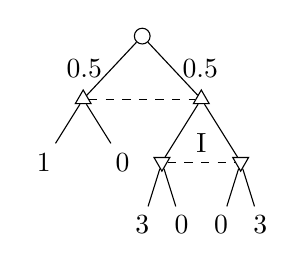
\begin{tikzpicture}
\node [ch] {}
    child{ node [ma] (i1_1) {} 
	    child{ node {1}}
    	    child{ node {0}}
    	    edge from parent node[left] {0.5}
    }
    child{ node [ma] (i1_2) {}
	    child{ node [mi] (i2_1) {}
			   child{ node {3}}
	    		   child{ node {0}}
			 }	    
	    child{ node [mi] (i2_2) {}
			   child{ node {0}}
	    		   child{ node {3}}
			 }
		edge from parent node[right] {0.5}
	};
\draw [dashed] (i1_1) -- (i1_2);
\draw [dashed] (i2_1) -- (i2_2) node[midway, above] {I};
\end{tikzpicture}
\end{center}
\caption{An extensive-form game demonstrating the problem of non-locality with maximizing $\bigtriangleup$, minimizing $\bigtriangledown$ and chance $\bigcirc$ players.
\label{fig:coordGame}}
\end{figure}

% Merge-Nov15; as far as I can tell I merged in your version with my small addition at the end.

We demonstrate the problem of non-locality on the game depicted in Figure~\ref{fig:coordGame}. The game starts with a decision of chance $\bigcirc$ which leads to to nodes than cannot be distinguished by the maximizing player $\bigtriangleup$. In the one on the left, the game ends after his actions. In the other one, both his actions lead to the information set $I$ of the minimizing player $\bigtriangledown$.
The optimal (Nash equilibrium) strategy in $I$ depends on the value of the leftmost leaf, even though this outcome of the game cannot be reached once the game entered the information set $I$.
Because $\bigtriangleup$ does not know at the time of his move if $\bigtriangledown$ will play, he needs to randomize its decision so that $\bigtriangledown$ cannot easily make the move that is more harmful for $\bigtriangleup$. However, he would prefer to play left for the case that $\bigtriangledown$ will not play. Player $\bigtriangledown$ knows that $\bigtriangleup$ has this dilemma and tries to exploit it as much as possible. The uniform strategy at $I$ clearly motivates $\bigtriangleup$ to play left, leading to expected utility $0.5\cdot 1 + 0.5\cdot1.5 = 1.25$, instead of $0.5\cdot 0 + 0.5\cdot1.5 = 0.75$. If $\bigtriangledown$ plays right a little more often, $\bigtriangleup$ is still motivated to play left and $\bigtriangledown$ improves its payoff. This holds until $\bigtriangledown$ plays (left,right) with probabilities ($\frac{1}{3}$,$\frac{2}{3}$). In that case $\bigtriangleup$ has the same expected reward of $1$ for both actions. If $\bigtriangleup$ plays $(\frac{1}{2},\frac{1}{2})$, $\bigtriangledown$ cannot lower the utility anymore and this pair of strategies is a Nash equilibrium. If the leftmost leaf was 2 instead of 1, the optimal strategy in $I$ would be ($\frac{1}{6}$,$\frac{5}{6}$).

%The optimal (Nash equilibrium) strategy for the game on the right is obtained by solving $\max_{\sigma_1 \in \Sigma_1} \min_{\sigma_2 \in \Sigma_2} u_1(\sigma_1, \sigma_2)$, which gives $\bigtriangleup$ to play $(\frac{1}{2},\frac{1}{2})$ and for $\bigtriangledown$ to play (left,right) with probabilities ($\frac{1}{3}$,$\frac{2}{3}$). The expected value of the game is $1$.

Current approaches, after reaching the information set $I$, will repeatedly sample and search one of subtrees of states in $I$, aggregating the information collected to make a final recommendation.
%When hidden information is revealed for search, Russel and Norvig refer to this technique as ``averaging over clairvoyance''~\cite{russellnorvig}.
However, even if the information structure is kept intact and information is aggregated during the searches, such as in Information Set Monte Carlo tree search (ISMCTS)~\cite{Cowling12ISMCTS}, the problem still occurs. If subtrees of $I$ are sampled equally often, a searching player will not have any preference between left and right and will recommend $(\frac{1}{2},\frac{1}{2})$, which is suboptimal.
% However, mixing uniformly at $I$ is not part of an equilibrium in this game. The payoff to $\bigtriangleup$ for playing right would be $\frac{1}{2}\cdot 0 + \frac{1}{2} \cdot \frac{3}{2} = \frac{3}{4}$, which would give $\bigtriangleup$ incentive to switch to play left more often (since its expected value is $\frac{5}{4}$), in turn giving $\bigtriangledown$ incentive to deviate. 
In this case, the uniform probability of being in each state of $I$ corresponds to the distribution over the states given the optimal play, so the problem occurs even if subtrees are sampled from the proper belief distribution. 
% this is mentioned later (after the proof)
% and no search algorithm starting only from the current match history $\ttm$ without some extra informaiton cannot converge to the optimal strategy.
Note that this is a simple example; in larger games, this problem could occur over much longer paths or in many times in different parts of the game.

%To overcome this problem, we propose a new approach. Instead of adapting perfect information search techniques to imperfect information games, we present online variants of Monte Carlo equilibrium approximation algorithms that have been successful in the offline setting.
OOS overcomes this problem by starting each sample from the root of the game. If the computed strategy tends to come closer to the uniform strategy in $I$ ,the updates in the maximizing player's information set will modify the strategy to choose left more often. It will cause the following samples to reach $I$ more often at the state on the left and consequently modifying the strategy in $I$ in the right direction in the following iterations.

To the best of our knowledge, OOS is the first online search algorithm that solves this problem. As suggested by the analysis in~\cite{Long10Understanding}, the effect may be critical in games with low {\it disambiguation factor}, where private information is very slowly (or never) revealed throughout a match.

\subsection{Offline Equilibrium Approximation}

There are many algorithms for computing approximate equilibrium strategies offline~\cite{Sandholm10The}. We focus on a popular choice among Poker researchers due to its sampling variants.

Counterfactual Regret (CFR) is a notion of regret at the information set level for extensive-form games~\cite{CFR}. 
The CFR algorithm iteratively learns strategies in self-play, converging to an equilibrium. 
The \defword{counterfactual value} of reaching information set $I$ is the expected payoff given that player $i$ played to reach $I$, the opponents played 
$\sigma_{-i}$ and both players played $\sigma$ after $I$ was reached:
\begin{equation}
\label{eq:cfv}
v_i(I,\sigma) = \sum_{(h,z) \in Z_I} \pi^{\sigma}_{-i}(h) \pi^{\sigma}(h,z) u_i(z), 
\end{equation}
where $Z_I = \{ (h,z)~|~z \in Z, h \in I, h \sqsubset z \}$.
Suppose, at time $t$, player $i$ plays with strategy $\sigma^t_i$. 
Define $\sigma^t_{I \rightarrow a}$ as identical to $\sigma^t$ except at $I$ action $a$ is taken with probability $1$. 
The counterfactual regret of not taking $a \in A(I)$ at time $t$ is $r^t(I,a) = v_i(I,\sigma^t_{I \rightarrow a}) - v_i(I,\sigma^t)$. 
The algorithm maintains the cumulative regret $R^T(I,a) = \sum_{t=1}^T r^t(I,a)$, for every action at every information set of every player. 
Then, the distribution at each information set for the next iteration $\sigma^{T+1}(I)$ is obtained individually using 
regret-matching~\cite{Hart00}. The distribution is proportional to the positive portion of the individual actions' regret:
\begin{equation*}
\label{eq:rm}
\sigma^{T+1}(I,a) = \left\{
\begin{array}{ll}
R^{T,+}(I,a) / R^{T,+}_{sum}(I) & \mbox{if } R^{T,+}_{sum}(I) > 0 \\ 
1 / |A(I)|                   & \mbox{otherwise,}
\end{array} \right.
\end{equation*}
where $x^+ = \max(0,x)$ for any term $x$, and $R^{T,+}_{sum}(I) = \sum_{a' \in A(I)} R^{T,+}(I,a')$. Furthermore, the algorithm maintains for each information set the average strategy profile
\begin{equation}
%\bar{\sigma}^T(I,a) = \frac{1}{T}\sum_{t=1}^T \sigma^t(I,a).
\bar{\sigma}^T(I,a) = \frac{\sum_{t=1}^T \pi^{\sigma^t}_i(I) \sigma^t(I,a)}{\sum_{t=1} \pi^{\sigma^t}_i(I)}, 
\end{equation}
where $\pi^{\sigma^t}_i(I) = \sum_{h \in I}\pi^{\sigma^t}_i(h)$.
The combination of the counterfactual regret minimizers in individual information sets also minimizes the overall average regret \cite{CFR}, and hence the average profile is a $2\epsilon$-equilibrium, with $\epsilon \rightarrow 0$
as $T \rightarrow \infty$.

Monte Carlo Counterfactual Regret Minimization (MCCFR) applies CFR to sampled portions of the games~\cite{Lanctot09Sampling}. 
In the \defword{outcome sampling} (OS) variant of the algorithm, a single terminal history $z\in Z$ is sampled in each iteration. 
The algorithm updates the regret in the information sets visited along $z$ using the 
\defword{sampled counterfactual value}, 
\begin{equation*}
\tilde{v}_i(I,\sigma) = \left\{
\begin{array}{ll}
\frac{1}{q(z)} \pi^{\sigma}_{-i}(h) \pi^{\sigma}(h,z) u_i(z) & \mbox{if } (h,z) \in Z_I\\
0  & \mbox{otherwise,}
\end{array} \right.
\end{equation*}
where $q(z)$ is the probability of sampling $z$. 
As long as every $z \in Z$ has non-zero probability of being sampled, $\tilde{v}_i(I,\sigma)$ is an unbiased estimate of $v(I,\sigma)$ 
due to the importance sampling correction ($1/q(z)$). For this reason, applying CFR updates using these sampled counterfactual values 
on the sampled information sets values also eventually converges to the approximate equilibrium of the game with high probability. 
The required number of iterations for convergence is much larger, but each iteration is much faster.

%In Poker, CFR and MCCFR have been used with much success as offline methods 
%for pre-computing approximate equilibria in abstract games~\cite{CFR,Johanson12CFRBR}; the same general 
%approach has also been used in Liar's Dice~\cite{Neller11,Lanctot12IR}. 

\section{Online Outcome Sampling}

When outcome sampling is used in the offline setting, data structures for all information sets are allocated and created 
before the first iteration starts. In each iteration, every information set that is sampled gets updated. 
We make two essential modifications to adapt outcome sampling to the online search setting.

{\bf Incremental Game Tree Building.} Before the match begins, only the very first (root) information set is added to memory. 
In each iteration, a single information set (at most) is added to the information set tree (memory) each iteration.
In particular, when an information set is reached that is not in memory, it is added to memory and then a default 
playout policy (\eg uniform random) takes over for the remainder of the simulation.
Along the playout portion (tail) of the simulation, information sets are not added to memory nor updated.
Along the tree portion (head) of simulation, information sets are updated as normal. 
This way, only the relevant information sets will be stored in the memory.

{\bf In-Match Search Targeting.}
Suppose several moves have been played since the start of the match leading to $\ttm$. 
Plain outcome sampling would continue to sample from the root of the game (not the current match history $\ttm$), entirely 
disregarding the region of the game space that the match has headed toward. 
Hence, the second modification we propose is directing the search towards the histories that are more likely to occur during the match currently played.
Note that the complete history is typically unknown to the players, who know only their information sets.
Furthermore, unlike in ISMCTS, OOS always runs samples from the root of the game tree, even with non-empty match history.

We now describe two specific targeting methods.

\subsection{Information Set Targeting (IST)}

Suppose the match history is $\ttm$. IST samples histories reaching the current information set ($I(\ttm)$), 
i.e., $(h,z) \in Z_{I(\ttm)}$, with higher probability than other histories.
The intuition is that these histories are particularly 
relevant since the searching player {\it knows} that one of these $z$ will describe the match at its completion. 
However, focusing {\it only} on these histories may cause problems because of the non-locality and the convergence guarantees are lost.

Consider again the game in Figure~\ref{fig:coordGame}. 
If the minimizing player knows it is in the information set $I$ and focuses all its search only to this information set for sufficiently long, she computes the suboptimal uniform strategy.
Any fixed non-zero probability of sampling the left chance action will 
eventually solve the problem. The regrets are multiplied by the reciprocal of the sampling probability; hence, they influence the strategy 
in the information set proportionally stronger if the samples are rare.

Note that previous methods, such as PIMC and ISMCTS, {\it always} target $I(\ttm)$, \ie with probability 1, and do not 
update predecessors of $I(\ttm)$. In contrast, in IST {\it all} information sets in memory reached during each iteration requires updating 
to ensure eventual convergence to an equilibrium.

\subsection{Public Subgame Targeting (PST)}

A \defword{public action} is an action in the ``public tree'' defined in \cite{12aamas-pcs}. Informally, an action is said to be public if it is observable by all players (e.g., bids in Liar's Dice and bets in Poker are public). Formally, an action $a$ is public, iff 
$\forall i, \forall I \in \cI_i, \forall h_1,h_2\in I: a\in h_1 \Leftrightarrow a\in h_2$.
For example, the extensive-form version of Rock, Paper, Scissors has two information 
sets $I_1 = \emptyset$ and $I_2 = \{ r, p, s \}$; it has no public actions, because each history in 
$I_2$ contains a single unique action (the unobserved ones taken by the first player).  

Given a history $h$, let $p(h)$ be the sequence of public actions along $h$ in the same order that they were taken in $h$. 
Define the \defword{public subgame} induced by $I$ to be the one whose terminal history set is
\[Z_{p,I(h)} = \{(h',z)~|~z \in Z, h' \in H, p(h') = p(h), h' \sqsubset z \}.\]
Now, suppose the match history is $\ttm$.
Public subgame targeting samples $z \in Z_{p,I(\ttm)}$ with higher probability than terminal histories outside this set.

A public subgame then, contains all the terminal histories consistent with the public actions played over the match and
each combination of private chance events for both players. So, in a game of two-player limit Texas Hold'em poker, suppose the nature decides on the private cards of the players,
the first player bets one chip and the second player calls. At this point, the public actions are: bet one chip and call. 
The public subgame described by $Z_{p,I(h)}$ contains every terminal history (including every combination of private chance 
outcomes for all players) with at least two public actions, whose first two public actions are: bet one chip and call.  

\begin{figure}[t]
\begin{center}
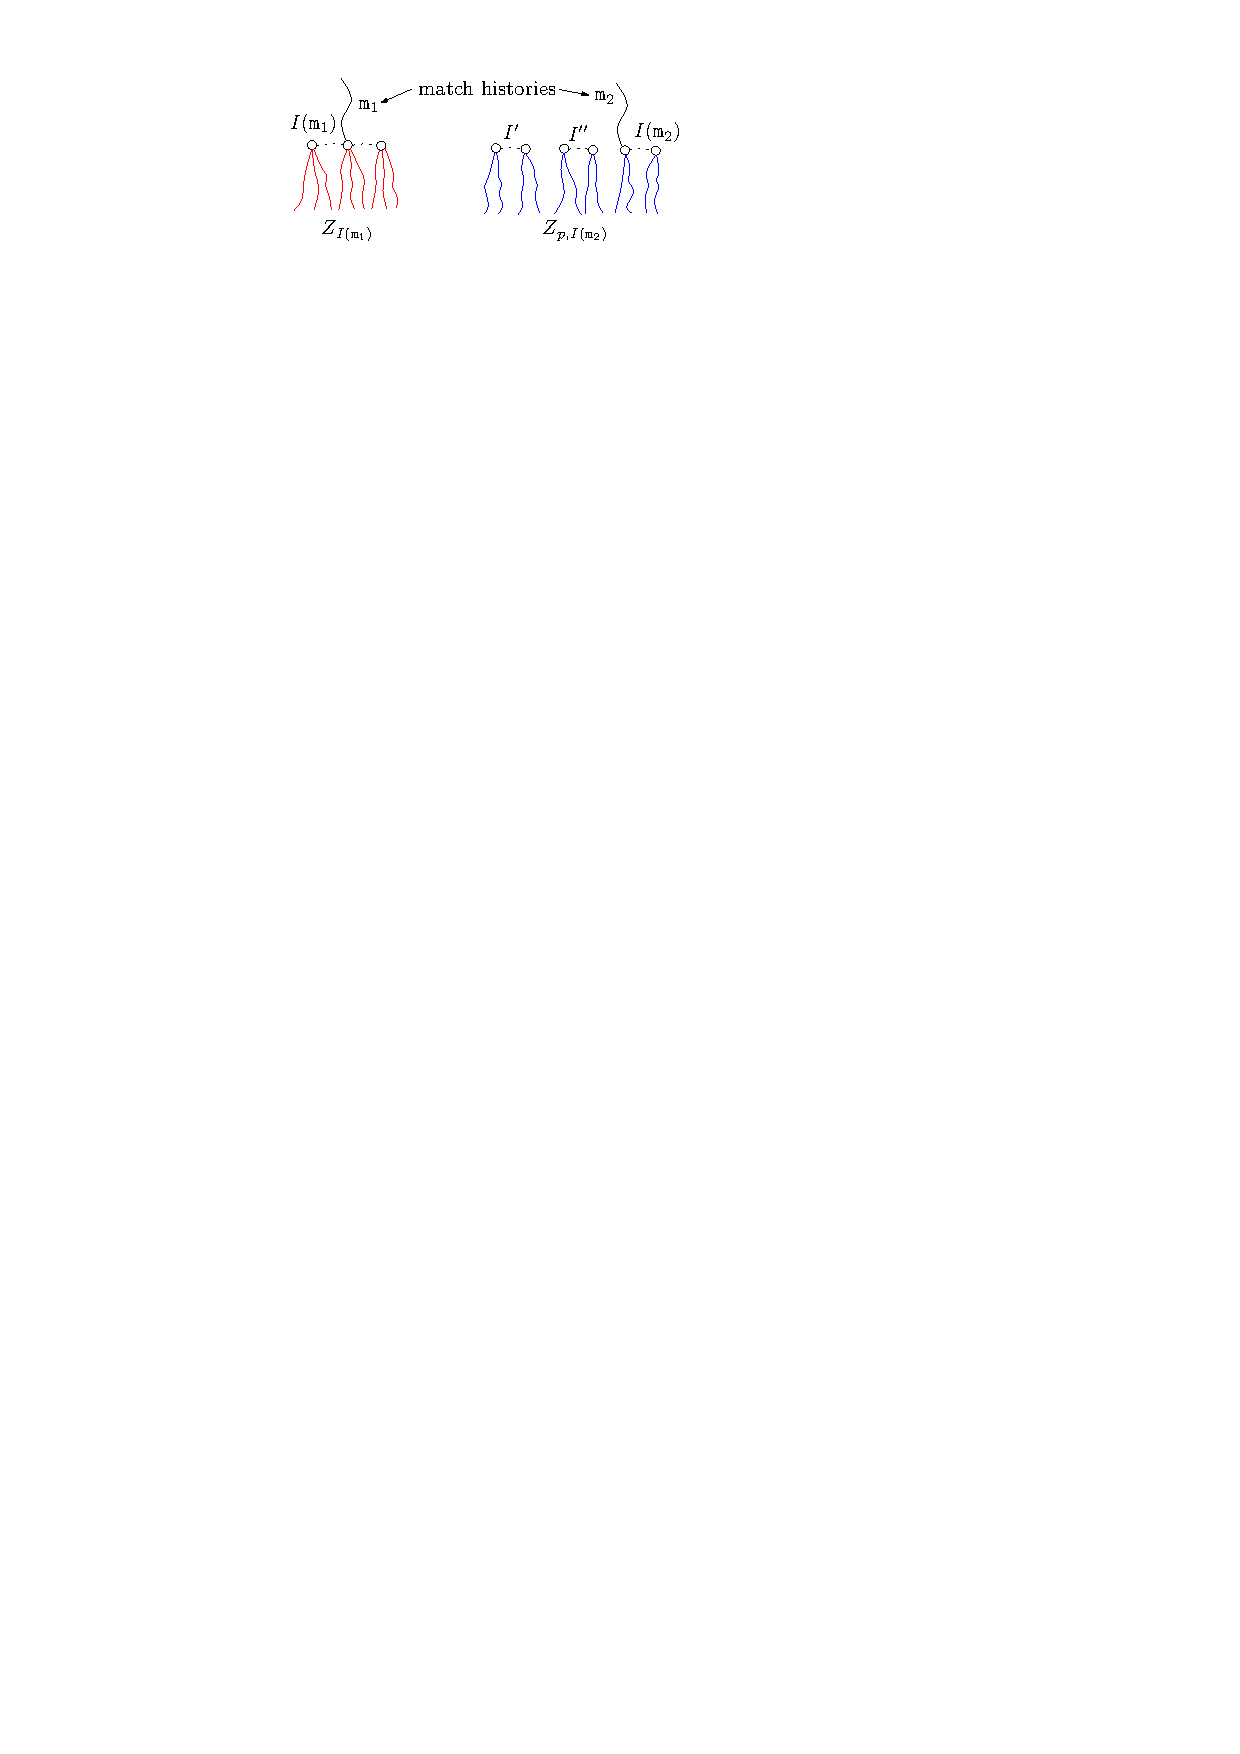
\includegraphics[scale=1.1]{fig/targeting}
\end{center}
\caption{Example subgames targeted by IST (left) and PST (right). All histories $\{~h~|~h \in I' \cup I'' \cup I(\ttm_2)~\}$ 
share a common public action sequence ($p(\ttm_2)$). \label{fig:targeting}}
\end{figure}

\subsection{Algorithm}


\begin{algorithm2e}[t]
  OOS$(h, \pi_i, \pi_{-i}, s_1, s_2, i)$: \; 
  \pushline
  \If{$h \in Z$}{
    \breturn $(1, \delta s_1 + (1-\delta)s_2, u_i(z))$\; \label{alg:terminal}
  }
  \ElsIf{$P(h) = c$}{
    Sample an outcome $a$ and let $\rho_1,\rho_2$ be its probability in targeted and untargeted setting \; \label{alg:chancesample}
    $(x, l, u) \gets $ OOS$(ha, \pi_i, \rho_2 \pi_{-i}, \rho_1 s_1 , \rho_2 s_2, i)$ \;
    \breturn $(\rho_2 x, l, u)$ \; 
  }
  $I \gets $ getInfoset$(h, P(h))$ \;
  Let $(a,s_1',s_2') \leftarrow $ Sample$(h, I, i, \epsilon)$ \; \label{alg:sample}
  \If{$I$ is not in memory}{ 
    Add $I$ to memory \;
    $\sigma(I) \leftarrow \mbox{Unif}(A(I))$ \;
    $(x, l, u) \gets $ Playout$(ha, \frac{\delta s_1 + (1-\delta)s_2}{|A(I)|})$ \; \label{alg:playout}
  }
  \Else{
    $\sigma(I) \gets $ RegretMatching$(r_I)$ \;
    $\pi_{P(h)}' \gets \sigma(I,a)\pi_{P(h)}$ \;    \label{alg:newreaches1}
    $\pi_{-P(h)}' \gets \pi_{-P(h)}$ \;             \label{alg:newreaches2}
    $(x, l, u) \gets$ OOS$(ha, \pi_i', \pi_{-i}', s_1', s_2', i)$ \;  
  }
  $c \gets x$ \;                   \label{alg:suffix1} 
  $x \gets x \sigma(I,a)$ \;     \label{alg:suffix2}
  \For{$a' \in A(I)$}{   
    \If{$P(h) = i$}{
      $W \gets u \pi_{-i}~/~l$ \;
      \If{$a' = a$}{
        $r_I[a'] \gets r_I[a'] + (c - x)W$ \;
      }
      \Else{
        $r_I[a'] \gets r_I[a'] - xW$ \;
      }
    }
    \Else{
      $s_I[a'] \gets s_I[a'] + \frac{1}{\delta s_1 + (1-\delta)s_2} \pi_{-i} \sigma(I,a')$ \;  \label{alg:avgstrat}
    }
  } 
  \breturn $(x, l, u)$ \;   \label{alg:returnend} 
  \popline
  \vspace{0.1cm}
  \caption{Online Outcome Sampling. \label{alg}}
\end{algorithm2e}

The algorithm is iterative and samples a single trajectory from the root $\emptyset$ to a 
terminal history. At each information set in memory, $I$, there are two tables maintained: $r_I$ stores cumulative 
regret for each action $a \in A(I)$, and $s_I$ stores the cumulative average strategy probability of each 
action. 

Depending on the targeting method that is chosen (IST or PST), $Z_{sub}$ is one of $Z_{I(\ttm)}$ or $Z_{p,I(\ttm)}$. 
The pseudo-code is presented as Algorithm~\ref{alg}. 
Each iteration is represented by two calls of OOS where the update player $i \in \{1,2\}$ is alternated. 
Before each iteration, a {\it scenario} is decided: 
with probability $\delta$ the iteration targets the subgame and chooses $z \in Z_{sub}$
and with probability $(1-\delta)$ the usual OS sampling determines $z \in Z$. 
The first parameter of OOS is the current history. 
The next two are strategy's reach probabilities for the update player $i$ and the opponent. 
The third and fourth parameters are initially the overall probabilities that the current sample is generated, one for each scenario: first the targeted and then the untargeted.
With non-empty match history, these two parameters include an additional weighting factor $w_T$ explained later.
The last parameter is the update player. Initial calls have the form OOS$(\emptyset, 1, 1, 1/w_T, 1/w_T, i)$.  
For the return values, $x$ is a suffix/tail reach probability for both players, 
$l$ is the root-to-leaf sample probability, and $u$ is the payoff of the trajectory in view 
of the update player. 

In outcome sampling, an $\epsilon$-on-policy sampling distribution used at each information set
is defined as 
\begin{equation*}
\label{eq:ossample}
\Phi(I,i) = \left\{
\begin{array}{ll}
\epsilon \cdot \mbox{Unif}(A(I)) + (1-\epsilon)\sigma_i(I) & \mbox{if } P(I) = i\\ 
\sigma_i(I)                                          & \mbox{otherwise,}
\end{array} \right.
\end{equation*}
and denote $\Phi(I,i,a)$ the probability of sampling $a \in A(I)$. 

The sampling at chance's choices on line~\ref{alg:chancesample} depends on the method and the scenario being used. For example, when using information set targeting, the outcome that is sampled must be consistent with match history.

A critical part of the algorithm is the action chosen and sample reach updates on line~\ref{alg:sample}. If $I$ is not in memory, then an action is sampled uniformly. Otherwise, in the targeted scenario, the current history $h$ is always in the targeted part of the game and an action from $\{a~|~\exists z\in Z \; (ha,z)\in Z_{sub}\}$ is selected using the distribution $\Phi(I(h),i)$ normalized to one on this subset of actions. If we define $sum=\sum_{(ha,z)\in Z_{sub}}\Phi(I,i,a)$ then $s_1' = s_1\Phi(I,i,a)/sum$. In the untargeted scenario, any action $a \sim \Phi(I,i)$ can be sampled. If the action is not leaving the targeted part of the game (i.e., $(ha,z)\in Z_{sub}$) then $s_1' = s_1\Phi(I,i,a)/sum$ otherwise $s_1'=0$. In all cases $s_2' = \Phi(I,i,a) s_2$.

These sample reach probabilities are combined into one at a terminal history on line~\ref{alg:terminal}, 
start of the playout on line~\ref{alg:playout}, and when updating the average 
strategy on line~\ref{alg:avgstrat}. 

The playout on line~\ref{alg:playout} samples to the end of the game with some playout policy at each step; we use uniform random, 
but in general one could use an informed policy based on domain knowledge as well. 
Unlike MCTS, the playout policy in OOS must compute $l$ when reaching a terminal and update the tail probability $x$ when returning
as done on line~\ref{alg:suffix2}. Lines~\ref{alg:newreaches1} and \ref{alg:newreaches2} modify $P(h)$'s reach probability 
by multiplying it by $\sigma(I,a)$, keeping the other value the same.
Lines~\ref{alg:suffix1} to 24
contain the usual outcome sampling updates. Note that regrets are updated at the 
update player histories, while average strategy tables at opponent histories. \\

% I am fine with not giving this a title, just a single line of whitespace

Now we explain the role of the weighting factor $w_T$. Note that on lines 22 and 28, the regret and strategy updates are multiplied by the reciprocal of the probability of sampling the sample leaf and the current state. 
Consider the updates in the current information set of the game $I_\ttm$. In the initial samples of the algorithm with empty match history, this information set was on average sampled with a very low probability $s_0$. Let's say that out of $10^6$ samples started from the root, 1000 samples reached this particular information set. In that case, $s_0=0.001$ and the regret updates caused by each of these samples were multiplied by $\frac{1}{s_0}=1000$.
Now the game has actually reached the history $\ttm$ and due to targeting, half of the next $10^6$ samples reach $I_\ttm$. It means that  $s'_0=0.5$ and the regrets will be multiplied only by 2.
As a results, the updated of the first (generally less precise) 1000 samples are all together weighted the same as the $5\times 10^5$ later samples, which makes it almost impossible to compensate for the initial errors.
In order to prevent this effect, we add the weighting factor $w_T$ to compensate the change of targeting and make each of the samples have similar weight. 
In our example, $w_T=\frac{s'_0}{s_0}$. More formally, when running the iterations from match history $\ttm$, we define the weighting factor as the probability of reaching $I(\ttm)$ without any targeting divided by the probability of reaching $I(\ttm)$ with the current targeting, assuming the players play according to the current mean strategy profile $\bar{\pi}$:
\[\frac{1}{w_T(\ttm)} =  (1-\delta) + \delta\frac{\sum_{(h,z)\in I(\ttm)} \bar{\pi}(h)}{\sum_{z\in Z_{sub(\ttm)}} \bar{\pi}(z)}.\]

OOS would quickly stop improving a strategy in information sets that are below an irrational move of the opponent ($\pi_{-i}=0$). This can not be avoided even if all samples are targeted to the information set. Therefore, we use a more explorative regret matching, 
$\sigma^{T+1}_\gamma(I,a) = \gamma/|A(I)| + (1-\gamma) \sigma^{T+1}(I,a)$, with $\gamma = 0.01$. 
This affects the worst-case regret bound at most by $\epsilon$ (due to the linearity of the expected utility), but allows for much better play.



\subsubsection{Consistency}

\begin{theorem}
Let $\bar{\sigma}^t_m(\delta,\ttm)$ be a strategy produced by OOS with scheme 1$m \in \{ \mbox{IST}, \mbox{PST} \}$ 
using $\delta < 1$ started from $\ttm$ run for $t$ iterations, with exploration $\epsilon > 0$.  
For any $p \in (0, 1], \varepsilon > 0$ there exists $t < \infty$ such that with 
probability $1-p$ the strategy  $\bar{\sigma}^t_m(\delta,\ttm)$ is a $\varepsilon$-equilibrium strategy. 
\label{thm:consistency}
\end{theorem}
\begin{proof}(Sketch) Each terminal history has nonzero probability of being sampled, eventually every information 
set will be contained in memory. The algorithm then becomes MCCFR with a non-uniform sampling scheme.
By \cite[Theorem 5]{Lanctot09Sampling} OOS minimizes regret with high probability. The additional weighting of all updates of the algorithm by the same constant has no influence on the computed average strategy and the strategies computed by regret matching, because it considers only relative proportions of the regrets.
\end{proof}

Note that due to non-locality, this consistency property cannot hold generally for any search 
algorithm that does not modify $\sigma(I)$ at previous $I(h)$ such that $h \sqsubset \ttm$. However, 
it is an open question as to whether any of the previous algorithms could be modified to ensure 
consistency.

\section{Empirical Evaluation}

We now compare the exploitability  and head-to-head performance
of OOS and ISMCTS on three fundamentally different imperfect games. % with different sources of imperfect information. 


\subsection{Information Set Monte Carlo Tree Search}
We compare to Information Set Monte Carlo tree search implemented in the same framework with similar data representations as OOS. ISMCTS runs MCTS samples as in a perfect information game, but uses common statistics computed for the whole information set and not individual states to select the next move. When initiated from non-empty match history, it starts samples uniformly from the states in the current informaiton set. We use two selection functions in our experiments. First, the commonly used UCT as suggested in \cite{Cowling12ISMCTS}. We use two time the maximal game ourcome as the exploration parameter $C$. In matches, we select the action with the highest number of iterations. For evaluating convergence, this would often have the maximum possible exploitability in the evaluated games. Therefore, we use the distribution given by the empirical frequencies for this part of evaluation. Second, we use Regret Matching (RM) as the selection strategy, because it has been shown to empirically perform better in many games \cite{Lisy14selection} and because it is based on the same principles that are behind CFR. For RM, we use exploration $0.2$, the mean strategy for evaluating exploitability and the samples form this strategy in head to head matches. In the following, we refer to ISMCTS with the corresponding selection function by only UCT/RM.

\subsection{Evaluating Performance}\label{sec:evaluating}

In games like Poker and Liar's Dice, it is often critical to play in such a way that the opponent 
cannot easily infer the private information. This explains partly why CFR-based methods have 
enjoyed so much success in the offline approach. 
In the online setting, however, since the tree is built incrementally, only partial strategies
are produced. 
We are unaware of any methods for assessing the worst-case exploitability of strategies 
produced by an online search algorithm. 
We therefore propose two new methods to approximate the exploitability of the produced strategies. 

% "full stitching" 
%\begin{table}
%{\small
%\begin{center}
%\begin{tabular}{ccccc}
%Algorithm     & Time & $\epsilon_1$ & $\epsilon_2$ & $\epsilon_\sigma$ \\
%\hline
%ISMCTS        & 1s   & 0.235  & 0.574  & 0.808 \\
%IST           & 1s   & 0.337  & 0.311  & 0.648 \\
%PST           & 1s   & 0.203  & 0.211  & 0.414 \\
%\hline
%ISMCTS        & 5s   & 0.251  & 0.548  & 0.799 \\
%IST           & 5s   & 0.229  & 0.295  & 0.524 \\
%PST           & 5s   & 0.148  & 0.125  & 0.273 \\
%\hline
%\end{tabular}
%\caption{LD(1,1) exploitability using full-stitching, $\delta = 0.9$.} 
%\label{tbl:fullstitching}
%\end{center}
%}
%\end{table}

% I modified the text here; also included the results in here, but hard to shorten it further.
% On second thought: I am not sure we can include this in the end. The numbers look odd because 
% they don't match with the rest. Leaving it out for now to save space. This might hurt us, 
% we should think about what to do here.

%There is a brute-force method to compute exploitability of an online search algorithm.  
%Enumerate every information set in the game in a topological order from the root, performing a $t$-second search 
%for each one (sampling histories using belief distributions from previous searches closer to the root), making sure 
%not to unfairly use any saved statistics other than the ones computed at searches from parent information sets. 
%This simulates every possible way the game can be played, and takes $O(t |I|)$ seconds. 
%The resulting exploitabilities in LD(6,1,1), with $\gamma = 0.9$, 1 second search time are 
%$0.808$, $0.648$, and $0.414$ for ISMCTS, IST, and PST, respectively. We repeated the experiment with 5 seconds search time, 
%and obtained $0.799$, $0.524$, and $0.273$, respectively, confirming that OOS results in lower exploitability as search time increases. 
%However, since the it requires constantly saving and reloading memory states and running both sides separately to avoid 
%bias from the opponent's algorithm, the experiment took several days and is impractical for larger games.

There is a brute-force method that runs the algorithms to reach each information set and computes exploitability of a strategy composed form strategies comuted for these information sets. However, it requires $O(t |I|)$ seconds for a single run and mupliple runs are requiired for statisticaly significant results.
Instead, we propose an approximate multi-match \defword{aggregate method}. 
It creates a global (accumulating) strategy data structure for each player.
Then, it runs a fixed number of matches (500 in our experiments) of the search algorithm against a random opponent. In each information set reached in the match, the information computed (visit counts in ISMCTS, $s_I$ in OOS) is added into the global strategy of the player who searched.
Besides the information in the current information set, the information computed in all successor information sets is also added with a weight proportional to the number of visits of the information set.
If an information set is never reached directly, this gives at least some estimate of how the strategy would behave there. If it is, the number of samples in the information set out-weights the less precise estimates from the cases where it does not.  In the information sets not added to the global strategy, a fixed random action is selected. The result is the exploitability of the global strategy.

%For a fair comparison, the first $I$ reached along each $m$ aggregates all the information gained in the search 
%but for future $I'$, only the information collected in each $I''$ reachable by $I'$ is aggregated.
% and generates a set of matches $M$. Then, each $m \in M$ is simulated invoking the appropriate search algorithm at each observed $I$ along $m$. 
%Since $m$ is predetermined, the choice made by the search algorithm is discarded, but the information computed (visit counts in ISMCTS, $s_I$ in OOS) is added into the global strategy data structure of the player who searched. 
%Note that it is safe to combine the information in this way: in ISMCTS the actions chosen and visits are independent of how $I'$ was reached. In OOS, the accumulating $s_I$ values of two converging $\epsilon$-equilibrium average strategies can be combined due to linearity of expected utility. 

\subsection{Domains}
\vlnote{comment on domain sizes}

\textbf{Imperfect Information Goofspiel II-GS($N$)} each player is
given a private hand of bid cards with values $0$ to $N-1$. A different
deck of $N$ point cards is placed face up in a stack.
On their turn, each player bids for the top point card by secreatly choosing a single card in their hand. 
The highest bidder gets the point card and adds the point total to their score, discarding
the points in the case of a tie. 
This is repeated $N$ times and the player with the highest score wins.
In, II-Goofspiel the players only discover who won or lost a bid, but not the bid cards played.
Also, we assume the point-stack is strictly increasing: 0, 1, $\ldots N-1$.
This way the game does not have non-trivial chance nodes, all actions are private and information sets have various sizes.

\textbf{Liar's Dice} LD($D_1$,$D_2$), also known as Dudo, Perudo, and Bluff is a dice-bidding game. 
Each die has faces \epsdice{1} to \epsdice{5} and a star $\star$. 
Each player $i$ rolls $D_i$ of these dice without showing them to their opponent.
Each round, players alternate by bidding on the outcome of all dice in play until one player ``calls liar'', 
\ie claims that their opponent's latest bid does not hold.
If the bid holds, the calling player looses; otherwise, she wins.
A bid consists of a quantity of dice and a face value.  
A face of $\star$ is considered wild and counts as matching any other face.
To bid, the player must increase either the quantity or face value of the current 
bid (or both).
All actions in this game are public. The only hidden information is caused by chance at the beginning of the game. Therefore, the size of all information sets is identical. 


\textbf{Generic Poker} GP($T,C,R,B$) is a simplified poker game inspired by Leduc Hold'em. First, both players are required to put one chip in the pot.
Next, Nature deals a single private card to each player, and the betting round begins.
A player can either \emph{fold} (the opponent wins the pot), \emph{check} (let the opponent make the next move), \emph{bet} (add some amount of chips, as first in the round), \emph{call} (add the amount of chips equal to the last bet of the opponent into the pot), or \emph{raise} (match and increase the bet of the opponent).
If no further raise is made by any of the players, the betting round ends, Nature deals one public card on the table, and a second betting round with the same rules begins.
After the second betting round ends, the outcome of the game is determined --- a player wins if: (1) her private card matches the table card and the opponent's card does not match, or (2) none of the players' cards matches the table card and her private card is higher than the private card of the opponent. If no player wins, the game is a draw and the pot is split.
The parameters of the game are the number of types of the cards ($T$), the number of cards of each type ($C$), the maximum length of sequence of raises in a betting round ($R$), and the number of different sizes of bets (i.e., amount of chips added to the pot) for \emph{bet}/\emph{raise} actions.
This game is similar to Liar's Dice in having only public actions. However, it includes additional chance nodes later in the game, which reveal part of the information not available before. Moreover, it has integer results and not just win/draw/loss.

\begin{figure*}[t]
\hskip0.3cm
\hfill 
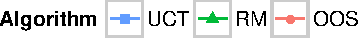
\includegraphics[height=3.5mm]{fig/legend_algs}
\hfill 

\includegraphics[height=3.5mm]{fig/legend_oos}
\hspace{0.8cm}

\rotatebox{90}{\hskip-1.5cm II Goofspiel (6)}
\subfigure[Root]{\label{fig:GS-root}
\begin{minipage}{0.235\textwidth}
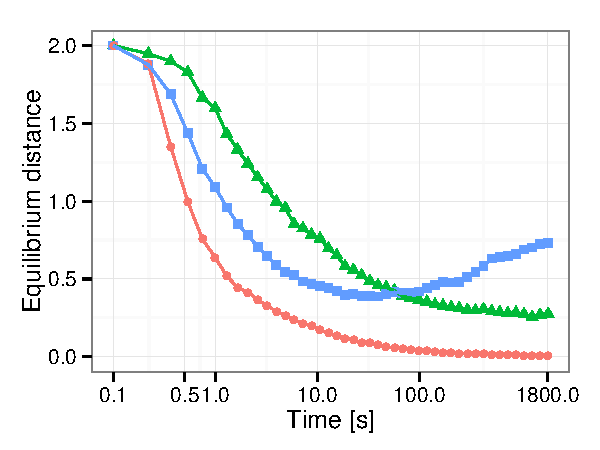
\includegraphics[width=\textwidth]{fig/convergence-IIGS_1_6}
\end{minipage}}
\subfigure[Aggregated]{\label{fig:GS-agg}
\begin{minipage}{0.235\textwidth}
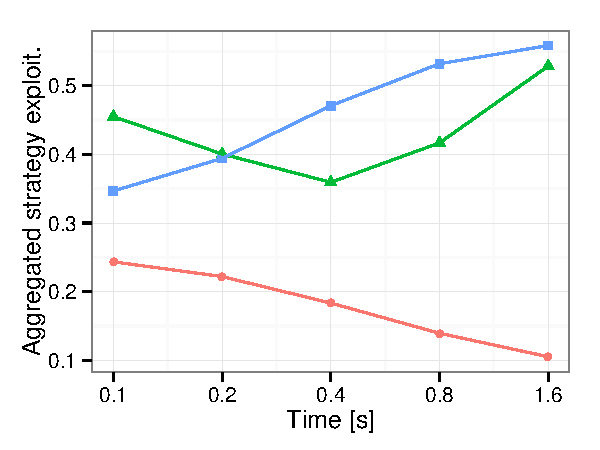
\includegraphics[width=\textwidth]{fig/agg_convergence-IIGS_1_6}
\end{minipage}}
\subfigure[OOS-IST Params.]{\label{fig:GS-oos}
\begin{minipage}{0.235\textwidth}
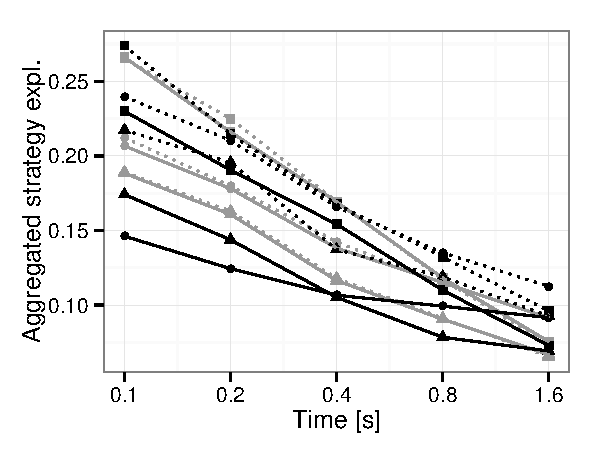
\includegraphics[width=\textwidth]{fig/agg_OSS-IST-WC_convergence-IIGS_1_6}
\end{minipage}}
\begin{minipage}{0.235\textwidth}
\center
No public subgame
\end{minipage}

\rotatebox{90}{\hskip-1.5cm Liar's Dice (6,1,1)}
\subfigure[Root]{\label{fig:LD-root}
\begin{minipage}{0.235\textwidth}
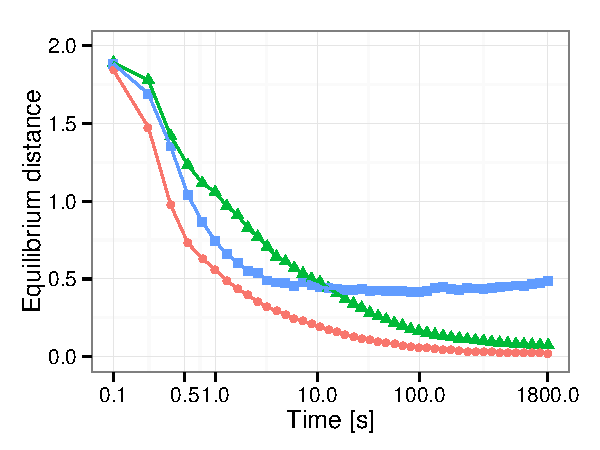
\includegraphics[width=\textwidth]{fig/convergence-LD_6_1_1}
\end{minipage}}
\subfigure[Aggregated]{\label{fig:LD-agg}
\begin{minipage}{0.235\textwidth}
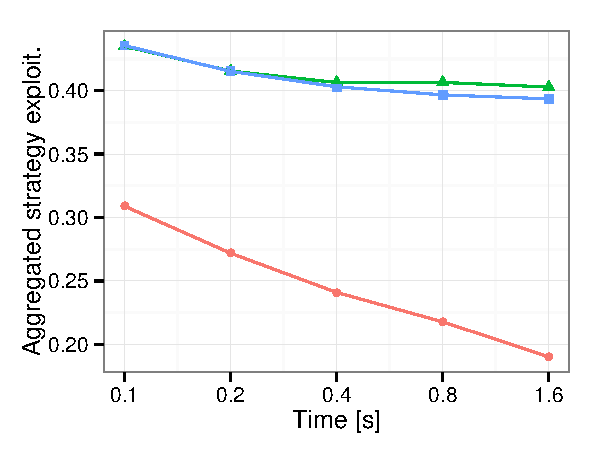
\includegraphics[width=\textwidth]{fig/agg_convergence-LD_6_1_1}
\end{minipage}}
\subfigure[OOS-IST Params.]{\label{fig:LD-IST-oos}
\begin{minipage}{0.235\textwidth}
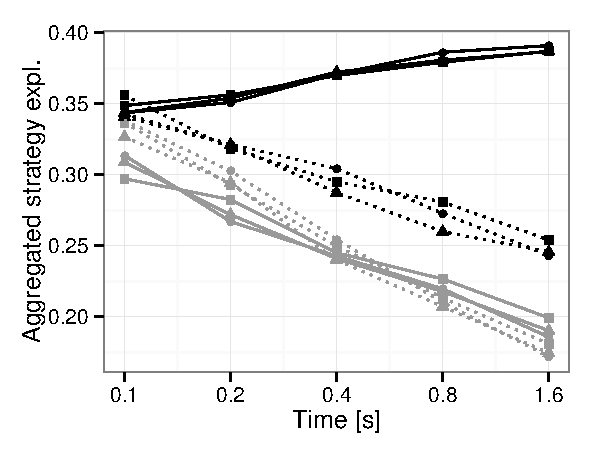
\includegraphics[width=\textwidth]{fig/agg_OSS-IST-WC_convergence-LD_6_1_1}
\end{minipage}}
\subfigure[OOS-PST Params.]{\label{fig:LD-PST-oos}
\begin{minipage}{0.235\textwidth}
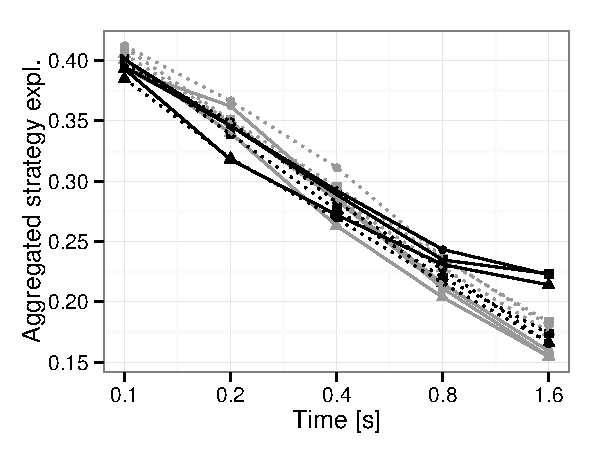
\includegraphics[width=\textwidth]{fig/agg_OSS-PST-WC_convergence-LD_6_1_1}
\end{minipage}}


\rotatebox{90}{\hskip-1.5cm Gen. Poker (3,3,2,2)}
\subfigure[Root]{\label{fig:GP-root}
\begin{minipage}{0.235\textwidth}
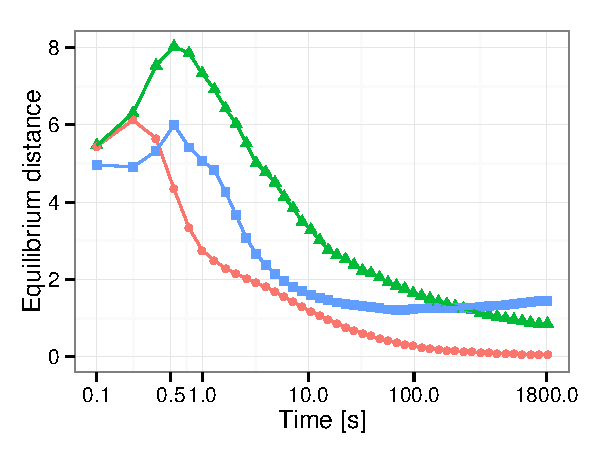
\includegraphics[width=\textwidth]{fig/convergence-GP_2_2_3_3}
\end{minipage}}
\subfigure[Aggregated]{\label{fig:GP-agg}
\begin{minipage}{0.235\textwidth}
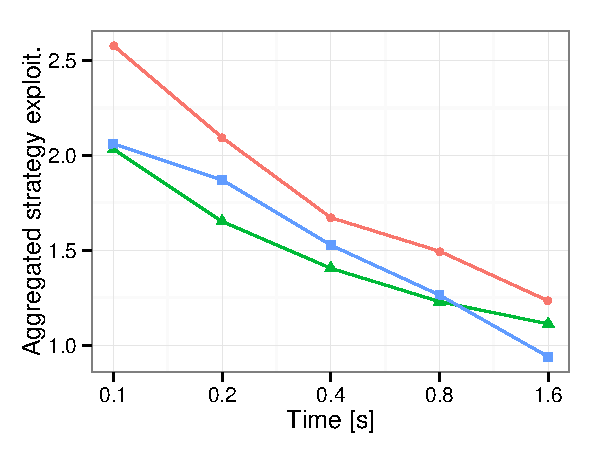
\includegraphics[width=\textwidth]{fig/agg_convergence-GP_2_2_3_3}
\end{minipage}}
\subfigure[OOS-IST Params.]{\label{fig:GP-oos-ist}
\begin{minipage}{0.235\textwidth}
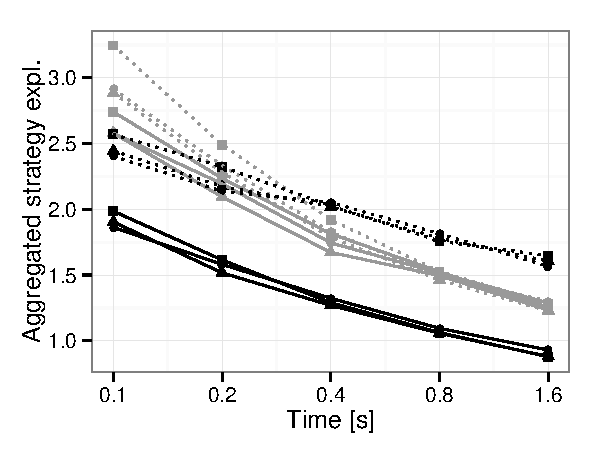
\includegraphics[width=\textwidth]{fig/agg_OSS-IST-WC_convergence-GP_2_2_3_3}
\end{minipage}}
\subfigure[OOS-PST Params.]{\label{fig:GP-oos-pst}
\begin{minipage}{0.235\textwidth}
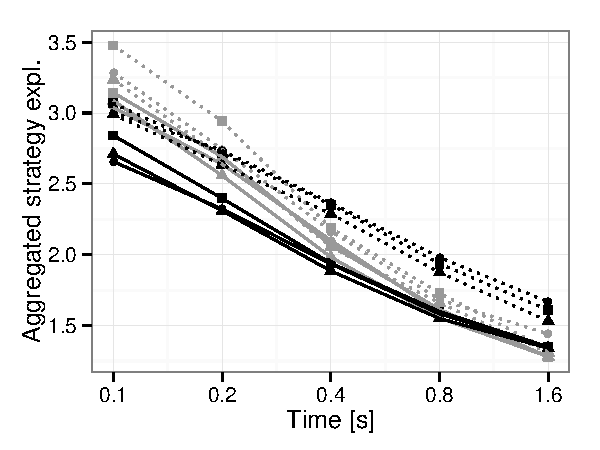
\includegraphics[width=\textwidth]{fig/agg_OSS-PST-WC_convergence-GP_2_2_3_3}
\end{minipage}}

\caption{Exploitability and head-to-head performance in small game variants. The values after $\pm$ at the matches are the maximum size of the 95\% confidence intervals over all values in the table. (d) and (h) are win rates, while (l) is the difference of the  expected outcome of a pair of strategies and the value of the game.}\label{fig:small}
\end{figure*}

\subsection{Results}

We first focus on LD(1,1), II-GS(6), and GP(3,3,2,2). While these games are considered small by search algorithm standards, it is still possible to compute the exact worst case counterstrategies (i.e., best response) to measure exploitability.  After analyzing the convergence, we proceed to performance in head-to-head matches with ISMCTS.

\subsubsection{Convergence at the root}

First we evaluate the speed of convergence of the proposed algorithm when run in the root of the games. The strategy in the information sets, which are not included in the tree yet, is assumed to be a fixed random action identical for all algorithms. The impact of the exploration parameters of the algorithms is not very strong here and we set it to $0.6$ for OOS. The results are in Figures~\ref{fig:small}(a,d,h). OOS clearly converges the fastest in all games, eventually converging to the exact equilibrium. The exact convergence is not surprising, because the algorithm run from the root is MCCFR, only with incremental tree building.

In all three games, the empirical action frequencies in UCT first converge quite quickly towards less exploitable strategies, but they always start to become more exploitable at some point. This does not happen with RM, but its initial convergence rate is smaller.

\begin{figure*}[t]
\subfigure[II Goofspiel (6)]{\label{fig:GS-matches-small}
\begin{scriptsize}
\begin{tabular}{@{}|@{}r@{}|@{~}c@{~}c@{~}c@{~}c@{}|}\hline
0.1s&OOS&UCT&RM&RND\\\hline
OOS&49.3(2.7)&50.0(1.3)&50.5(1.3)&83.1(1.5)\\
UCT&51.2(2.2)&62.9(2.6)&62.7(2.5)&84.0(2.1)\\
RM&52.3(1.4)&70.6(1.7)&73.1(2.1)&87.8(1.4)\\
RND&17.1(2.2)&15.7(2.2)&10.3(1.8)&49.7(3.0)\\
\hline
\end{tabular}
\end{scriptsize}}
\subfigure[Liar's Dice (1,1)]{\label{fig:LD-matches-small}
\begin{scriptsize}
\begin{tabular}{@{}|@{}r@{}|@{~}c@{~}c@{~}c@{~}c@{}|}\hline
0.1s&OOS&UCT&RM&RND\\\hline
OOS&48.5(2.0)&51.7(2.0)&56.8(2.8)&83.3(1.5)\\
UCT&45.7(2.0)&49.7(2.0)&52.9(2.8)&87.2(1.3)\\
RM&47.9(2.8)&49.0(2.8)&54.3(2.8)&84.8(2.0)\\
RND&16.9(1.5)&19.5(1.6)&18.1(2.2)&47.7(2.0)\\
\hline
\end{tabular}
\end{scriptsize}}
\subfigure[Generic Poker (3,3,2,2)]{\label{fig:GP-matches-small}
\begin{scriptsize}
\begin{tabular}{@{}|@{}r@{}|@{\hspace{1pt}}c@{~}c@{~}c@{~}c@{}|}\hline
0.1s&OOS&UCT&RM&RND\\\hline
OOS&0.25(0.53)& -0.45(0.10)& -0.40(0.10)& 1.85(0.16)\\
UCT& 0.53(0.10)&0.21(0.15)&0.20(0.15)&1.35(0.36)\\
RM& 0.39(0.13)&0.21(0.40)&-0.12(0.32)&1.75(0.44)\\
RND& -2.17(0.20)&-2.22(0.54)&-3.24(0.55)&1.07(0.61)\\
\hline
\end{tabular}
\end{scriptsize}}

\subfigure[II Goofspiel (13)]{\label{fig:GS-matches-large}
\begin{scriptsize}
\begin{tabular}{@{}|@{}r@{}|@{~}c@{~}c@{~}c@{~}c@{}|}\hline
1s&OOS&UCT&RM&RND\\\hline
%OOS&49.5(3.1)&25.4(2.7)&21.2(2.5)&72.8(2.7)\\
OOS&49.2(2.5)&28.3(3.9)&35.1(4.2)&83.0(3.2)\\
UCT&69.2(4.0)&70.0(2.8)&61.0(3.0)&90.6(1.8)\\
RM&67.5(4.0)&73.8(2.7)&67.5(2.9)&92.8(1.5)\\
RND&19.6(3.4)&6.2(1.5)&4.9(1.3)&49.0(3.0)\\
\hline
\end{tabular}
\end{scriptsize}}
\subfigure[Liar's Dice (2,2)]{\label{fig:LD-matches-large}
\begin{scriptsize}
\begin{tabular}{@{}|@{}r@{}|@{~}c@{~}c@{~}c@{~}c@{}|}\hline
5s&OOS&UCT&RM&RND\\\hline
OOS&49.9(3.7)&55.4(2.3)&53.3(3.7)&91.3(1.7)\\
UCT&49.8(2.2)&56.2(3.1)&49.8(3.1)&93.7(1.5)\\
RM&53.3(3.5)&51.7(4.0)&51.0(4.0)&88.7(2.0)\\
RND&7.3(1.6)&12.9(2.1)&12.7(2.1)&47.3(3.0)\\
\hline
\end{tabular}
\end{scriptsize}}
\subfigure[Generic Poker (4,6,4,4)]{\label{fig:GP-matches-large}
\begin{scriptsize}
\begin{tabular}{@{}|@{}r@{}|@{~}c@{~}c@{~}c@{~}c@{}|}\hline
1s&OOS&UCT&RM&RND\\\hline
OOS&-0.54(0.47)&-1.79(0.27)&-2.19(0.32)&8.36(0.54)\\
UCT&-0.07(0.35)&0.22(0.10)&-0.76(0.18)&9.48(0.40)\\
RM&-0.12(0.38)&-0.28(0.17)&-0.97(0.22)&9.09(0.44)\\
RND&-3.25(0.43)&-3.91(0.27)&-4.12(0.31)&2.51(0.51)\\
\hline
\end{tabular}
\end{scriptsize}}
\caption{Head-to-head matches in small (a-c) and large (d-f) variants of the games. Computation time per move is indicated in top left corner and half of 95\% confidence intervals in the brackets.}\label{fig:matches}
\end{figure*}


\subsubsection{Aggregated strategy exploitability}

Figures~\ref{fig:small}(b,e,i) present the exploitability of the strategies computed by different algorithms estimated by the aggregate method.% explained in Section~\ref{sec:evaluating}.
The OOS in this graphs is run with the information set targeting and the parameters $\gamma=0.4$ for exploration and $\delta=0.5$ for targeting.
The x-axis denotes the amount of computation per move.
In Goofspiel (b), both ISMCTS variants  produce a more exploitable strategy with more computation time per move.
For any of the evaluated time settings, OOS is substantially less exploitable.
In Liar's Dice (e), ISMCTS does not seem to get worse with additional computation time, but it improves marginally with more than $0.4$ second per move.
OOS steadily approaches the equilibrium.
In Poker (i), the exploitability is lower for ISMCTS variants than for OOS with the default settings.
With the limited computation time, having more iterations to avoid bad moves seems to be more important than guessing and hiding the private information of the players.

The remaining plots in Figures~\ref{fig:small} present how the exploitability of the strategies produced by OOS depends on the selected targeting scheme and parameters: the amount of targeting shown by color and the amount of exploration shown by point shapes. Figures \ref{fig:small}(c,f,j) show the information set targeting and \ref{fig:small}(g,k) show the public subgame targeting. Overall, OOS produces strategies closer to the equilibrium as the computation time per move increases. The only exception is IST with full targeting ($\delta=1$) in Liar's Dice (Figure~\ref{fig:LD-IST-oos}). This confirms that sampling the histories that will certainly not occur in the game anymore is necessary to converge to the optimal strategy in LD.
In the other two games, full targeting produces the least exploitable strategies with very short computation times. This indicates that sophisticated modeling of hidden information can be counterproductive with very short computation times. With more time per move, weaker targeting performs as good as the stronger targeting or even better in case of PST.

\vlnote{the next paragraph can be removed to save space}
%With short computation times, IST converges closer to the equilibrium, but with more computation, PST eventually dominates, with the exception of $\delta=1$ in Poker.
%In LD, PST is much less sensitive to the choice of parameters.
%The public subgame includes most of the relevant information.
%However, the sudden drop of the convergence speed of full targeting around 1s per move indicates that the public subgame does not contain all the relevant information.

% Removed to estimate space
%\begin{itemize}
%\item the game playing performance in large game with limited time is bad. This is likely because the targeting costs a lot of computational resources and the untargeted portions of the tree are not visited/updated enough to fix the strategies anyway.
%\end{itemize}

\subsubsection{Head-to-head performance}

After we confirmed that we achieved the goal of creating an online game playing algorithm that converges close to Nash equilibrium, we evaluate its game playing performance in head-to-head matches with ISMCTS.
For each game, we focus on two sizes. The smaller variant, for which we analyzed the exploitability in the previous section and a substantially larger variant that is closer to the size of the domains where online search algorithms are typically applied. 

%Game values
%LD611 -0.02713178294573644

%GP 2 2 3 3 -0.11135308803867544
%GP 4 4 4 6 -0.11123854182232012

The results are summarized in Figure~\ref{fig:matches}.
For Goofspiel and Liar's Dice, we present the win-rate, where a tie is considered half win half loss. GS is perfectly balanced for both players. In LD, the first player has a slight disadvantage corresponding to approximately 1\% \mlnote{...?} in the win rate and we do not compensate for that.
Poker is not balanced. If both players play the optimal strategy, the first player looses 0.11 chips on average.
This value is practically the same for both evaluated sizes of the game.
For clarity, we present the difference between this game value and the mean reward obtained by the players in the matches. A value 0.1 in the tables means that the row player on average wins 0.1 more than the game value from the comumn player per match.
Each entry in the tables presents the result of at least 500 mutual matches between two algorithms from the perspective of the one in the row header. The values in the brackets are the size of half of the 95\% confidence intervals centered in the presented mean. If it is not specified otherwise, OOS was run with IST for Goofspiel and PST for the other games, targeting $\delta=0.9$ and exploration $\epsilon=0.4$.

Figure~\ref{fig:GS-matches-small} presents the results for the smaller Goofspiel and $0.1$ second of computation per move. Even though the game is balances, the results of ISMCTS are strongly biased towards the first player. The second player has generally larger information sets and needs to better evaluate the hidden information  to choose a good move. OOS does not have this problem in the smaller game. It is the only algorithm that managed to prevent ISMCTS from exploiting it.
In both positions, the algorithm won approximately 50\% of matches, which corresponds to the value of the game.
On the other hand, the first line in the table shows that OOS did not exploit the weaker play of ISMCTS, even though it is possible. This is a common disadvantage of Nash equilibrium play. % quite well known ..? do we need a cite? \cite{}
One simple way to overcome this would be to trade a bit of exploitability to gain some exploitation; computing a restricted Nash response using  MCRNR~\cite{Ponsen11Computing} (a minor modification of MCCFR) allows the best possible trade-off for a given importance between exploitability and exploitation. 
In the large variant of Goofspiel (see Figure~\ref{fig:GS-matches-small}) with one second per move, the situation is different. OOS does not manage to converge sufficiently close to the equilibrium and ISMCTS exploits it from both positions to a similar extent. Increasing the computation time to 5 seconds per move helps OOS to win 35\% matches against UCT, but it would likely need a substantially longer time to reach the equilibrium.

The results on Liar's Dice are even more promising for OOS. In the smaller game with $0.1$ second per move (Figure~\ref{fig:LD-matches-small}), OOS statistically significantly wins over both variants of ISMCTS form at least one position. This is not the case for the larger game and 1 second per move, where OOS already wins only 45\% and 40\% of matches against UCT and RM from the first position and looses 69\% and 66\% from the second position. 
However, with 5 seconds and the exploration parameter set to $\epsilon=0.8$ to balance the need for exploring a large number of actions in this game, OOS again wins over UCT and ties with RM (Figure~\ref{fig:LD-matches-large}).

As indicated by the exploitability results, OOS performs the worst against ISMCTS in the Poker domain. In the smaller variant (Figure~\ref{fig:GP-matches-small}), it is losing from both positions. The result of OOS from the first position against UCT improves to ??? with 5 seconds per move and -0.28 with 25 seconds, but even more time would be required to tie. From the first (generally more difficult) position, the situation is similar also in the larger Poker (Figure~\ref{fig:GP-matches-large}). It is already not the case for the second position, were OOS is able to tie with both ISMCTS variants. 
This could be because Poker playing requires low-variance updates since the game itself already has high variance. 


% Removing this so I know how much trimming needs to be done.
%\begin{itemize}
%\item Without enough time for convergence, OOS has a lot of  (uniform) noise in the results. Focussing on top 3 actions with the corresponding probabilities may work better. In contrast ISMCTS with much more samples can easily get zeros at really bad actions. This could be solved by playing according to the current strategy!!! The expected strategy is optimal, but we do not even have to store the mean strategy!!! However, this may require some correct weighting (i.e., belief) that may not be available.
%\end{itemize}



\section{Conclusion}

\mlnote{Still needs expanding.}
We have introduced Online Outcome Sampling, the first online game playing algorithm for imperfect information games that is guaranteed to produce  
approximate equilibrium strategies as search time per move increases.
In order to achive this, we do not modify a perfect information search algorithm to avoid the main problems caused by imperfect informaiton, as in previous work.
We rather start from an offline equilibrium computation method and adapt it to make the most of the limited time it has by using the information about the current position in the match.
Besides incremental tree building, we propose two methods for targeting relevant parts of the game based on the current match history.
In empirical evaluation, we show that a player using ISMCTS can suffer almost arbitrarly large loss when the opponent knows the algorithm she uses. 
The expected worst-case loss of using OOS decreases close to its minimum with additional search time.
Furthermore, even with this guarantees, we can achieve comparable game playing performance to ISMCTS in mutual matches.

In future work, we hope to investigate more and larger games and the effect of informed playout policies. 
We hope to compare practical performance against other baseline algorithms such as 
PIMC~\cite{Long10Understanding}, MMCTS~\cite{Auger11Multiple}, IIMC~\cite{Furtak13Recursive}, and Smooth UCT~\cite{Heinrich14}.
Finally, one interesting question is whether the subgame decomposition ideas of~\cite{Burch14Solving,Jackson14} could be 
adapted to the online search setting. 

%\vlnote{ISMCTS often plays in support and it is hard to exploit it with NE play, even though the strategy can be completely exploitable. RNR may be a solution}

%ACKNOWLEDGMENTS are optional
%\section{Acknowledgments}
%This section is optional; it is a location for you
%to acknowledge grants, funding, editing assistance and
%what have you.  In the present case, for example, the
%authors would like to thank Gerald Murray of ACM for
%his help in codifying this \textit{Author's Guide}
%and the \textbf{.cls} and \textbf{.tex} files that it describes.

%
% The following two commands are all you need in the
% initial runs of your .tex file to
% produce the bibliography for the citations in your paper.
\bibliographystyle{abbrv}
\bibliography{iioos}  % sigproc.bib is the name of the Bibliography in this case
% You must have a proper ".bib" file
%  and remember to run:
% latex bibtex latex latex
% to resolve all references
%
% ACM needs 'a single self-contained file'!
%
%APPENDICES are optional
%\balancecolumns
%\appendix
%Appendix A
\end{document}
